\subsection{The Growth Impatience Conditions}

We have just shown that if the {\RIC} holds but the {\FHWC} does not, then the {\GICNrm} may not hold.  An illustration of such a case is provided in figure \ref{fig:FVACnotGIC}.

Consider again the \{\RIC,\cncl{\FHWC}\} case considered above under a configuration of parameters where the {\GICRaw} is satisfied but the {\GICNrm} is on the border between being satisfied and not being satisfied
\begin{align}
  \PGro \InvEpShkInv & = \Pat < \PGro
\\ \InvEpShkInv & = \Pat/\PGro < 1                       
\end{align}


If both the \GICNrm~and the \RIC~hold, the arguments above establish that as $\mRat \uparrow \infty$ the limiting consumption function asymptotes to the consumption function for the perfect foresight unconstrained function.

The more interesting case is where the \GICNrm~fails.
\begin{comment}
  \WW{}{The same
    steps as above lead to the same implication that this requires
    $\InvEpShkInv < (\Rfree/\PGro)^{1/\CRRA}\uInvEpShkuInv^{1-1/\CRRA}$,
    but when the \RIC~$\Rfree/\PGro > 1$ holds this condition is much more
    easily satisfied.}
  If the \FVAC~holds but the \GICNrm~does not, the parameters must satisfy:
  \begin{align}
    \DiscFac \PGro^{1-\CRRA}\Ex[\pshk^{1-\CRRA}] & < 1 < (\Rfree\DiscFac)^{1/\CRRA}(\PGro\Ex[\pshk^{-1}])^{-1}. \label{eq:FVACnotGIC}
  \end{align}

  Note first that by Jensens's inequality $\Ex[\pshk^{1-\CRRA}] > 1$ and $(\Ex[\pshk^{-1}])^{-1} < 1$,
  so \eqref{eq:FVACnotGIC} is stronger than
  \begin{align}
    \DiscFac \PGro^{1-\CRRA} & < 1 < (\Rfree\DiscFac)^{1/\CRRA}/\PGro. \label{eq:PFFVACnotGICRaw}
  \end{align}


  Suppose $\PGro=1$, $\CRRA=2$ and $\pshk$ is lognormally distributed with $\sigma^{2}_{\pshk}=0.01$ (that is, $\log \pshk \sim \mathcal{N}(-\sigma_{\pShk}^{2}/2,\sigma_{\pShk}^{2})$) so that $\Ex_{t}[\pshk_{t+1}^{1-\CRRA}] =\Ex_{t}[\pshk_{t+1}^{-1}] =\exp(\sigma^{2}_{\pShk})=e^{0.01}.$  Then the condition becomes
  \begin{align}
    \DiscFac e^{0.01} & < 1 < (\Rfree \DiscFac)^{1/2}e^{-0.01}
  \end{align}
  which can be satisfied, for example, by $\DiscFac = 0.96$ and $\Rfree=1.08$.
\end{comment}
A solution that satisfies the combination \FVAC~and
\cncl{\GICNrm} is depicted in Figure \ref{fig:FVACnotGIC}.  The
consumption function is shown along with the $\Ex_{t}[\Delta
\mRat_{t+1}]=0$ locus that identifies the `sustainable' level of
spending at which $\mRat$ is expected to remain unchanged.  The
diagram suggests a fact that is confirmed by deeper analysis: Under
the depicted configuration of parameter values (see the code for details), the consumption function never reaches the
$\Ex_{t}[\Delta \mRat_{t+1}]=0$ locus; indeed, when the \RIC~holds but
the \GICNrm~does not, the consumption function's limiting slope
$(1-\Pat/\Rfree)$ is shallower than that of the sustainable consumption
locus $(1-\PGroAdj/\Rfree)$,\footnote{This is because
  $\Ex_{t}[\mRat_{t+1}]=\Ex_{t}[\Rnorm_{t+1}(\mRat_{t}-\cRat_{t})]+1$; solve $\mRat = (\mRat - \cRat)\Rnorm \InvEpShkInv^{-1}+1$ for $\cRat$ and differentiate.}
so the gap between the two \textit{increases} with $\mRat$ in the
limit.  Although a nondegenerate consumption function
exists, a target level of $\mRat$ does not (or, rather, the
target is $\mRat=\infty$), because no matter how wealthy a consumer
becomes, the consumer will always spend less than the amount that
would keep $\mRat$ stable (in expectation).

\renewcommand{\figFile}{FVACnotGIC}
\hypertarget{\figFile}{}
\hypertarget{FVACnotGIC}{}
\begin{figure}[tbp]
\centerline{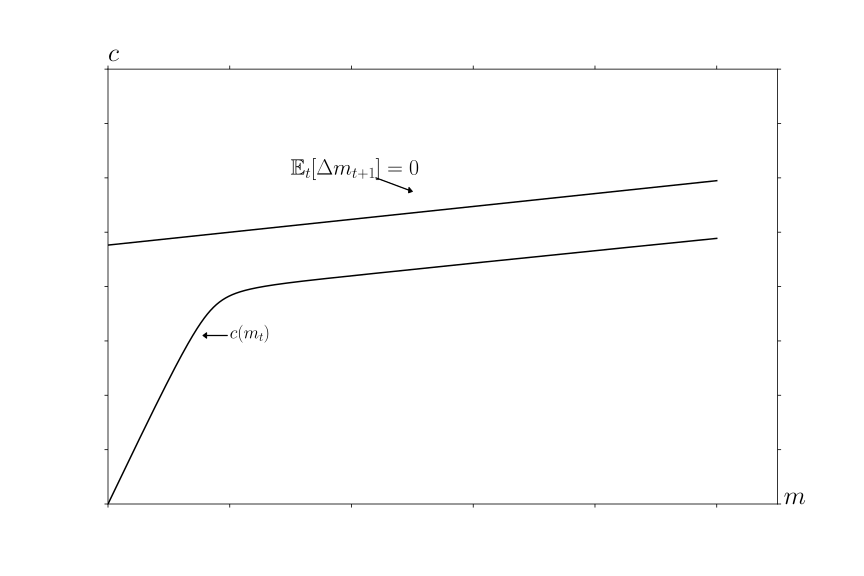
\includegraphics[width=6in]{\FigDir/FVACnotGIC}}
\caption{Example Solution under \{\FVAC,\cncl{\GICNrm}\}}
\label{fig:FVACnotGIC}
\end{figure}


\begin{comment}
  The foregoing has some connection with the theoretical results in
  Szeidl~\citeyearpar{szeidlInvariant}, who shows that the condition we
  call the \GICNrm~guarantees that $\mRat$ will have an asymptotically
  bounded mean.  He also shows that under these circumstances $\mRat$
  satisfies conditions he proves to be necessary for the existence of a
  stable invariant distribution.  Furthermore, $\aRat$, $\bRat$, and $\cRat$
  are also shown to have stable invariant distributions and asymptotically
  bounded means.  We make use of these results below.
\end{comment}

\begin{comment} % Not really necessary
  A final point worth reemphasizing is that neither the Return
  Impatience Condition nor the Finite Human Wealth Condition was
  required for the contraction mapping proof.  Both these conditions are
  necessary for a nondegenerate solution to exist in the unconstrained
  perfect foresight case.  This is noteworthy because in some models and
  in many economists' intuition, the introduction of uncertainty reduces
  the space of parameter values for which a unique solution exists;
  here, precisely the opposite occurs.  Indeed, many of the
  parameterizations newly eligible for solution are quite plausible, so
  this observation is not merely a curiosum but of real practical
  value.\footnote{An easy example of a case where the perfect foresight
    model has no solution is where $\Rfree >1$, $\DiscFac = 1/\Rfree$
    and $\PGro > \Rfree$.}
\end{comment}

\subsubsection{When the \GICNrm~Fails but the \GICRaw~Holds}\label{sec:WhenTheGICNrmFailsButGICRawHolds}

A particularly interesting case arises when human wealth is finite, the {\RIC} holds, but the normalized version of the GIC fails.

With finite human wealth and the {\RIC}, we know that
\begin{enumerate}
\item The perfect foresight solution to the non-normalized version of the problem exists;
\item The addition of uncertainty cannot increase the level of consumption;
  \item The solution to the model with uncertainty asymptotes to the solution to the perfect foresight model
  \end{enumerate}

  Interestingly, we therefore know that there must come a point at which $\Ex_{t}[\cLevBF_{t+1}]/\cLevBF_{t}] < \PGro$, and similarly for M.  
